\chapter{Guidelines for using the TABLe}
\label{appendix:TABLe_manual}

\section{OMRON Pump-down Procedure}

Special thanks for Andrew Piper for coding and installing the \OMRON safety system. Below is an operational guideline to pump the system down to UHV using the \OMRON system. Please see Andrew Piper's \OMRON manual for additional details on the microcontroller system.

This procedure assumes that the chambers are initially at atmospheric pressure, the rough pumps are turned on, and the solenoid shutoff valves on the roughing line are closed.

\begin{enumerate}
	\item Seal and isolate all chambers. Close the manual hand valves between each turbo pump and the solenoid shutoff valves. Reattach any blow-off flanges (KF-25 blanks) that may have come off from the previous venting cycle.
	\item Ensure the \OMRON's \, safety system is engaged by attempting to open one of the pneumatic gate valves via the control panel. \textbf{Caution: operating a gate valve between two chambers with a pressure differential can cause catastrophic system failure! Only perform this step after you have verified that all chambers are at atmospheric pressure!} If the gate valve opens while both chambers are above the upper setpoint, then the \OMRON \, safety system has been disabled. Enable the safety system by switching the override switch to OFF.
	\item Retract the metal filters from the beam path to protect them from potential pressure surges. 
	\item Initiate the pump-down sequence by pressing the OK button on the \OMRON. This will open all solenoid valves simultaneously with a loud \textit{thunk!}
	\item Slowly open the manual handvalves while monitoring the pressure load on the rough pumps to avoid overloading the rough pump system. Use the two Raspberry Pi remote pressure monitoring systems to monitor the inlet pressure for each blower system. As a rule of thumb, try to keep the inlet pressure below $\approx$100 Torr during this step. \textbf{Warning: overloading the rough pumps will result in pump oil being expelled into the rough pump's exhaust line. Continuing to run in this condition can lead to overheating and eventually seizing of the rough pump.}
	\item Once the hand valves are fully open on all chambers, you can turn each blower system ON to accelerate the remaining pump-down procedure.
	\item Power on the turbo power supplies and switch the turbos to ON. After a few seconds, the magnetically levitated turbos will start levitating with a soft \textit{thunk!}.
	\item Each turbo will automatically start spinning when its chamber reaches the upper set point (about 200 mTorr). The turbos will take a few minutes to reach their final speed.
	\item Wait for the system to pump down. It typically takes 15-45 minutes for the entire system to reach $10^{-6}$ Torr.
	\item The pneumatic gate valves for adjacent chambers will be enabled when both chambers are below their lower setpoint pressure (about $5 \times 10^{-6}$ Torr). Once all chambers are below their lower setpoints, the \OMRON considers the system is to be fully pumped down.
	\item ARM each chamber by pressing ESC + [chamber number]. The \OMRON's display will update to show which chambers are armed (G: generation \& differential pump chambers, M: mirror chamber, T: target chamber, S: photon spectrometer chamber).
\end{enumerate}

\section{OMRON Venting Procedure}

The \OMRON \ system was designed with the ability to vent any single chamber or combination of chambers while keeping the others pumped down. This was a possibility when each chamber had its own rough pump, but now that the mirror, target \& spectrometer chambers share a single blower system, extra care must be taken. \textbf{Any chambers that share a backing rough pump must be vented simultaneously to avoid turbopump overload.} For example, the mirror chamber, target chamber and spectrometer share a common blower system, and attempting to vent the one chamber while keeping the others will result in the spectrometer's turbo pump crashing due to the high backing pressure in the rough line.

This procedure assumes an initial condition of all chambers pumped down to UHV with the turbos running.

\begin{enumerate}
	\item Turn off all gas sources / loads. If the HPC is installed, follow the HPC shutdown procedure.
	\item Turn off the blowers.
	\item Block the laser into the interferometer.
	\item Close the pneumatic gate valves.
	\item Disarm the chambers by pressing ESC + [chamber number].
	\item Verify the \OMRON's safety system is not disabled by checking the bypass switch.
	\item Enable the venting valves by switching ON the vent \& purge controls on the control panel. The chambers will not vent without this step!
	\item Remove the KF clamps on the blow-off valves.
	\item Start the \OMRON \ venting script by pressing ALT + [chamber number] on the \OMRON.
	\item The user can now walk away from the system. It will take a few hours to vent.
\end{enumerate}

The venting script will immediately stop the turbopump's motors, open the solenoid venting valves after 30 seconds, close the roughing line's solenoid valves after 30 minutes, and close the solenoid venting valves after about 5 hours. The preceding timeline was chosen following the manufacturer's recommendation, and to avoid closing the roughing line's valves before the turbos had completely stopped spinning. 

\section{Aligning the Interferometer}
\label{app:aligning-interferometer}

\subsection{the generation arm}

\subsubsection{The Ellipsoidal Mirror}

\subsection{the pump arm}

\subsection{finding spatial overlap}

\subsection{finding temporal overlap}

\section{Pointing into the Interferometer}
\label{app:pointing-into-TABLE}

the importance of pointing into the interferometer - spatial and temporal alignment

\section{The High Pressure Cell (HPC)}

\begin{figure}
	\centering
	\includegraphics[width=0.9\textwidth]{figures/app1/HPC_outside_view.png}
	\caption{Exterior view of the generation chamber with the HPC installed showing the ancillary vacuum hardware. Red arrow indicates input laser path; green arrow points towards the HPC's RV pump.}
	\label{fig:HPC_outside_view}
\end{figure}

\begin{figure}
	\centering
	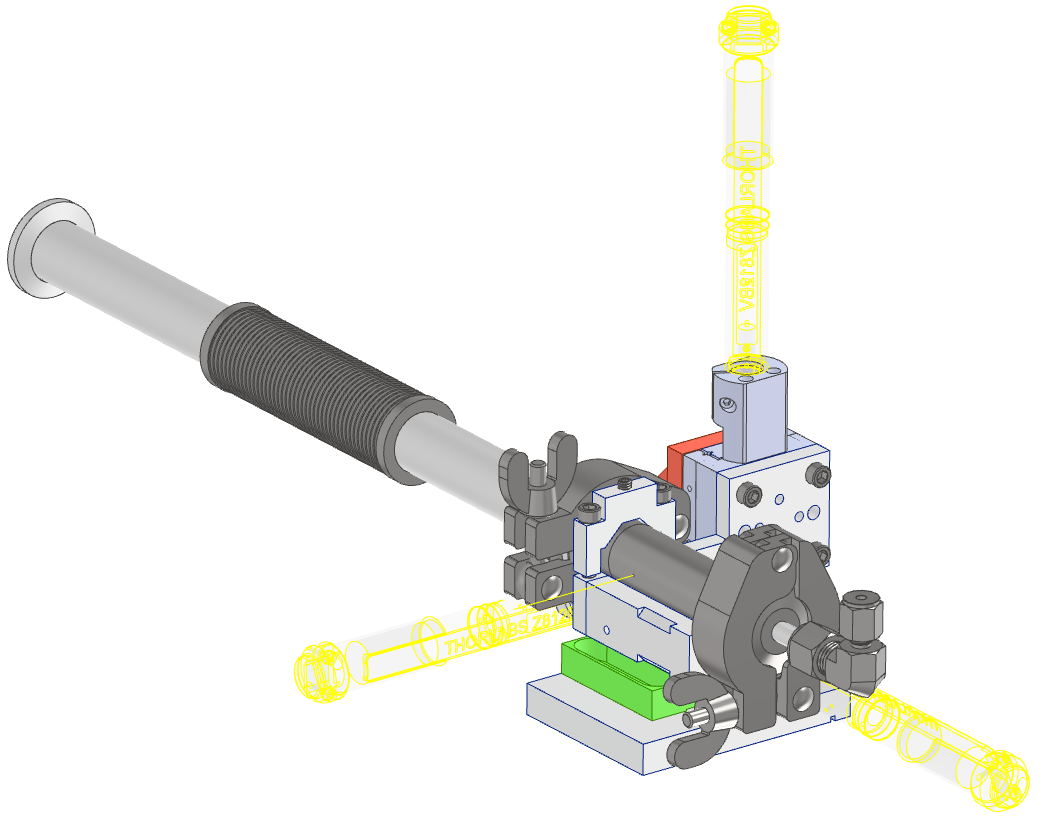
\includegraphics[width=0.9\textwidth]{figures/app1/HPC_on_stage2.png}
	\caption{The HPC with bracket installed on the XYZ translation stage, configured for the generation chamber. The hose clamp and gas supply tube is omitted from this drawing for clarity.}
	\label{fig:HPC_on_stage}
\end{figure}

\begin{figure}
	\centering
	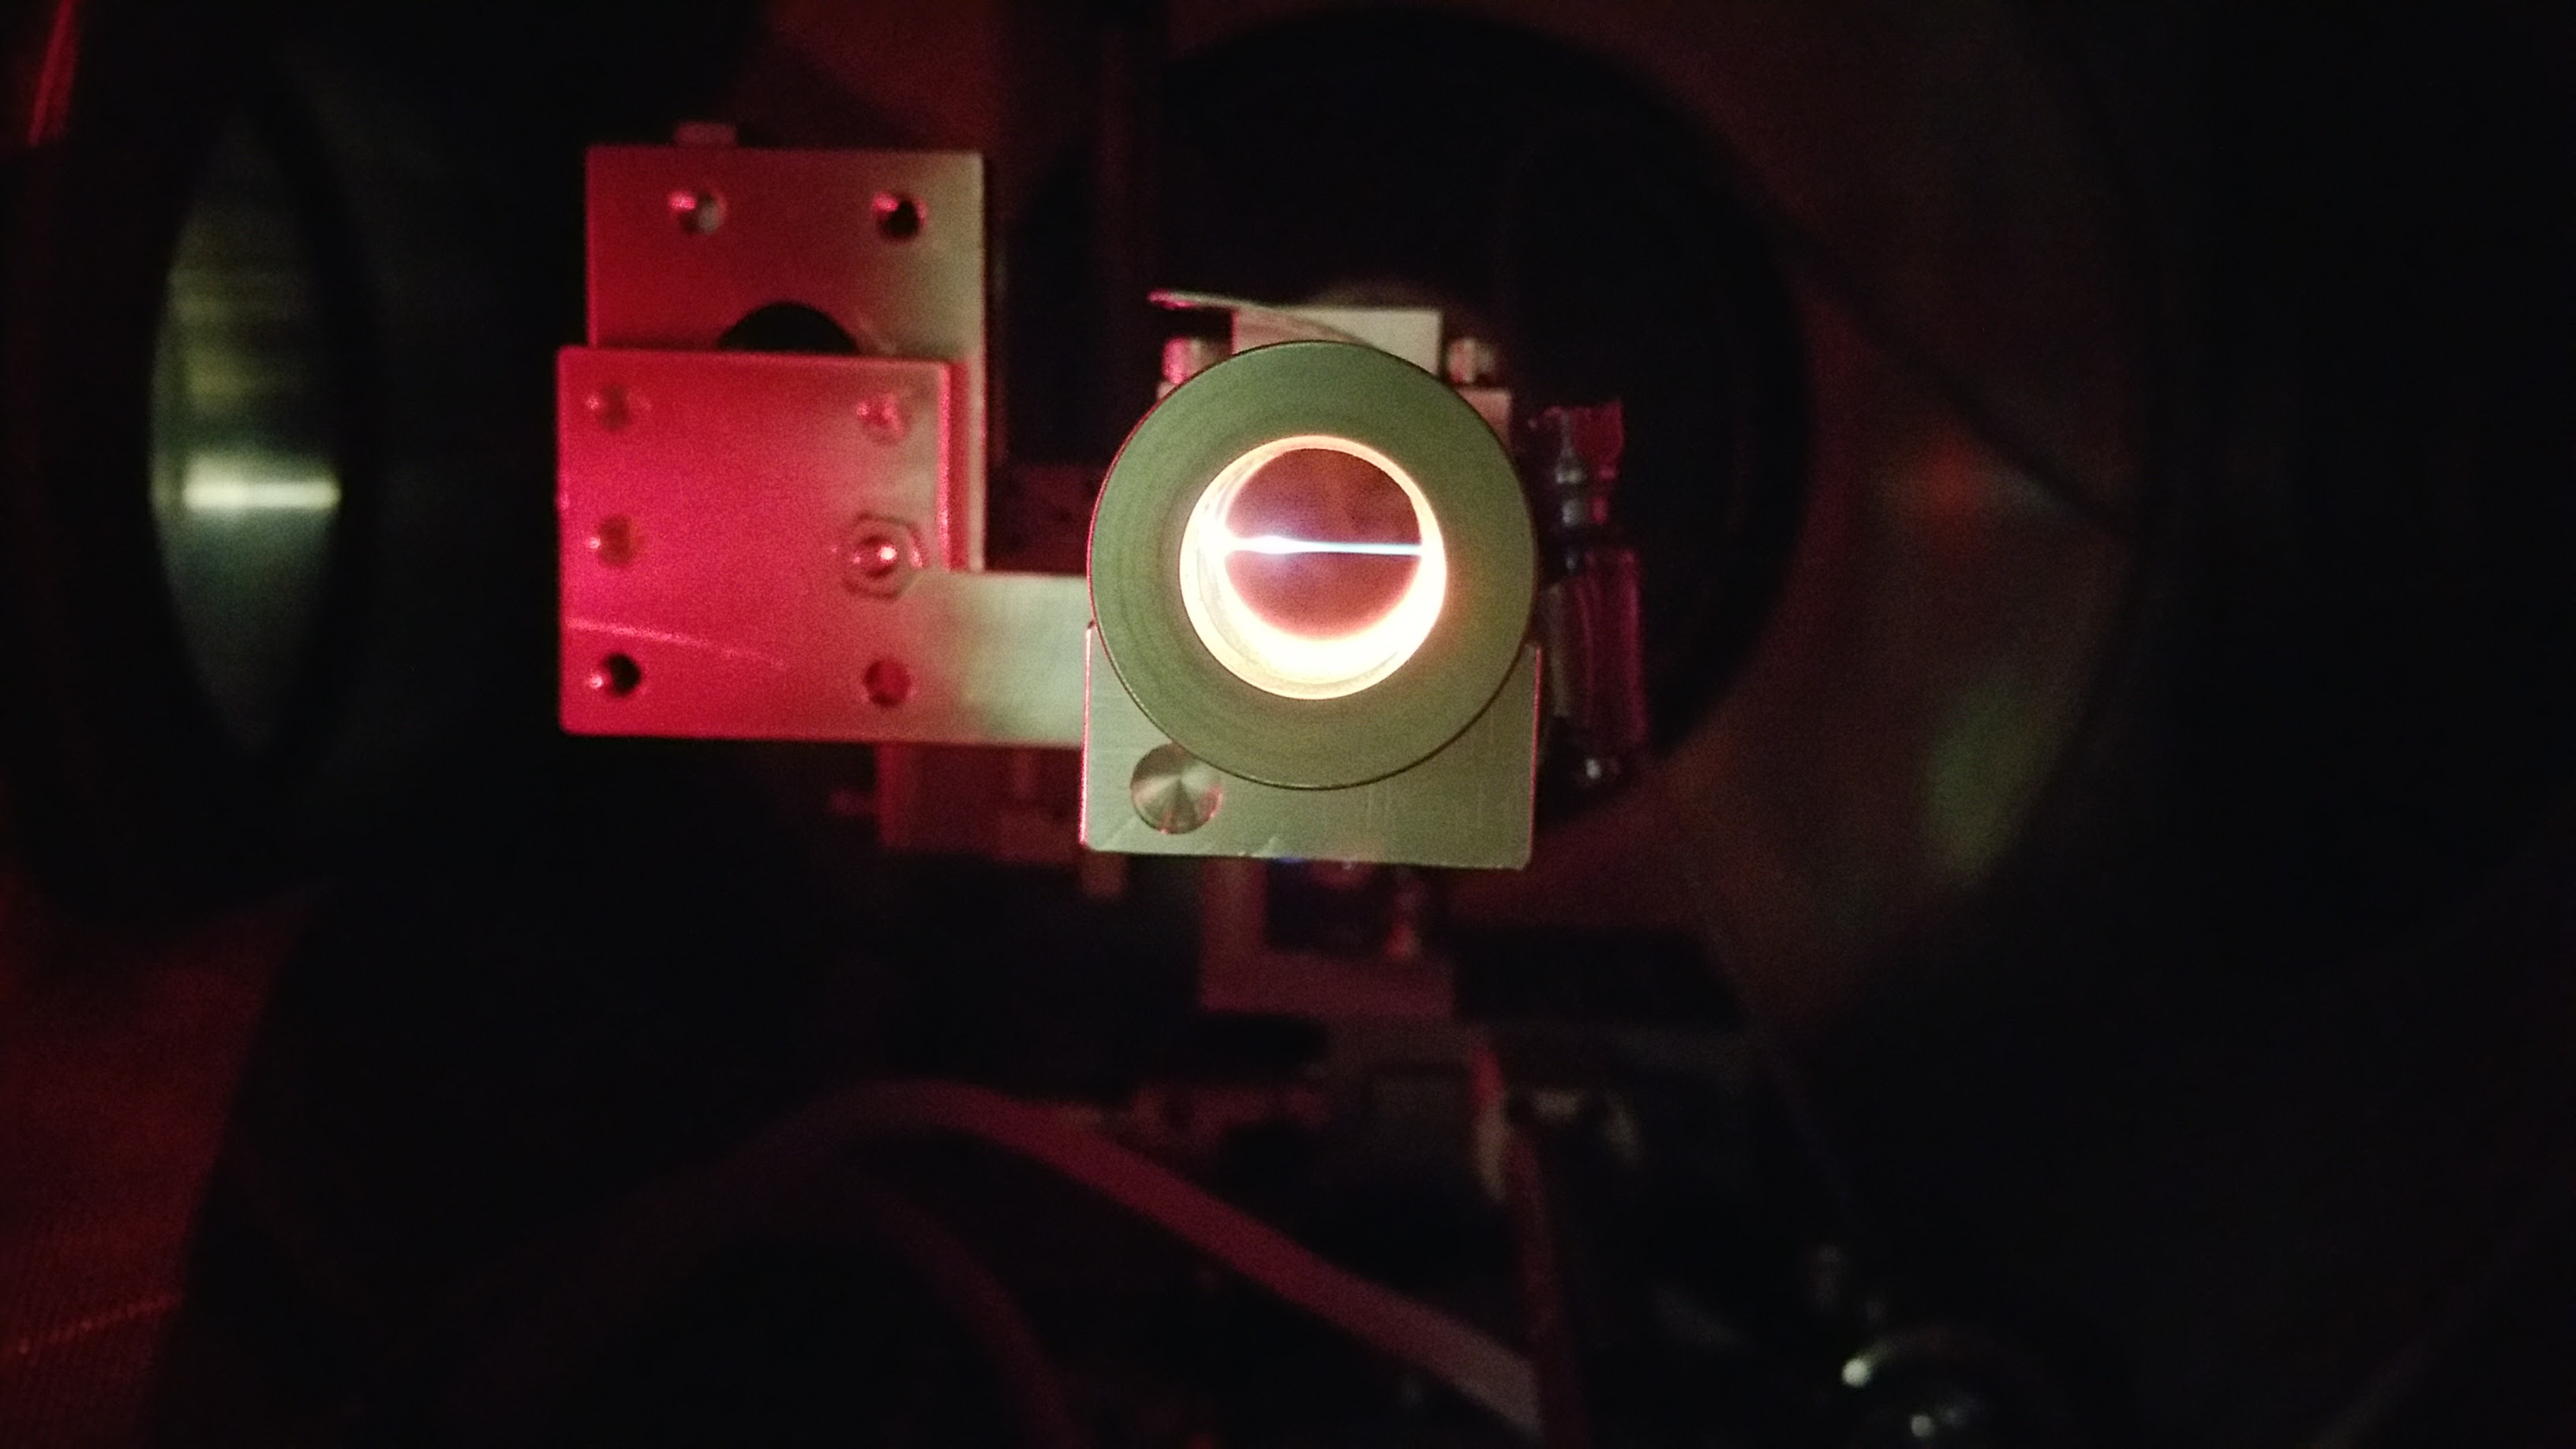
\includegraphics[width=0.75\textwidth]{figures/app1/HPC_outer_can_laser.jpg}
	\caption{Laser filament in the aligned outer pipe of the HPC. The inner pipe is not yet installed. Alignment of the outer pipe is done at very low intensities; after alignment the power was increased to create a filament for illustrative purposes only. This picture was taken in the target chamber during the initial testing of the HPC. The geometry of this chamber requires that the orientation of the mounting bracket is reversed compared to what is shown in Fig \ref{fig:HPC_on_stage}.}
	\label{fig:HPC_outer_can_laser}
\end{figure}

\begin{figure}
	\centering
	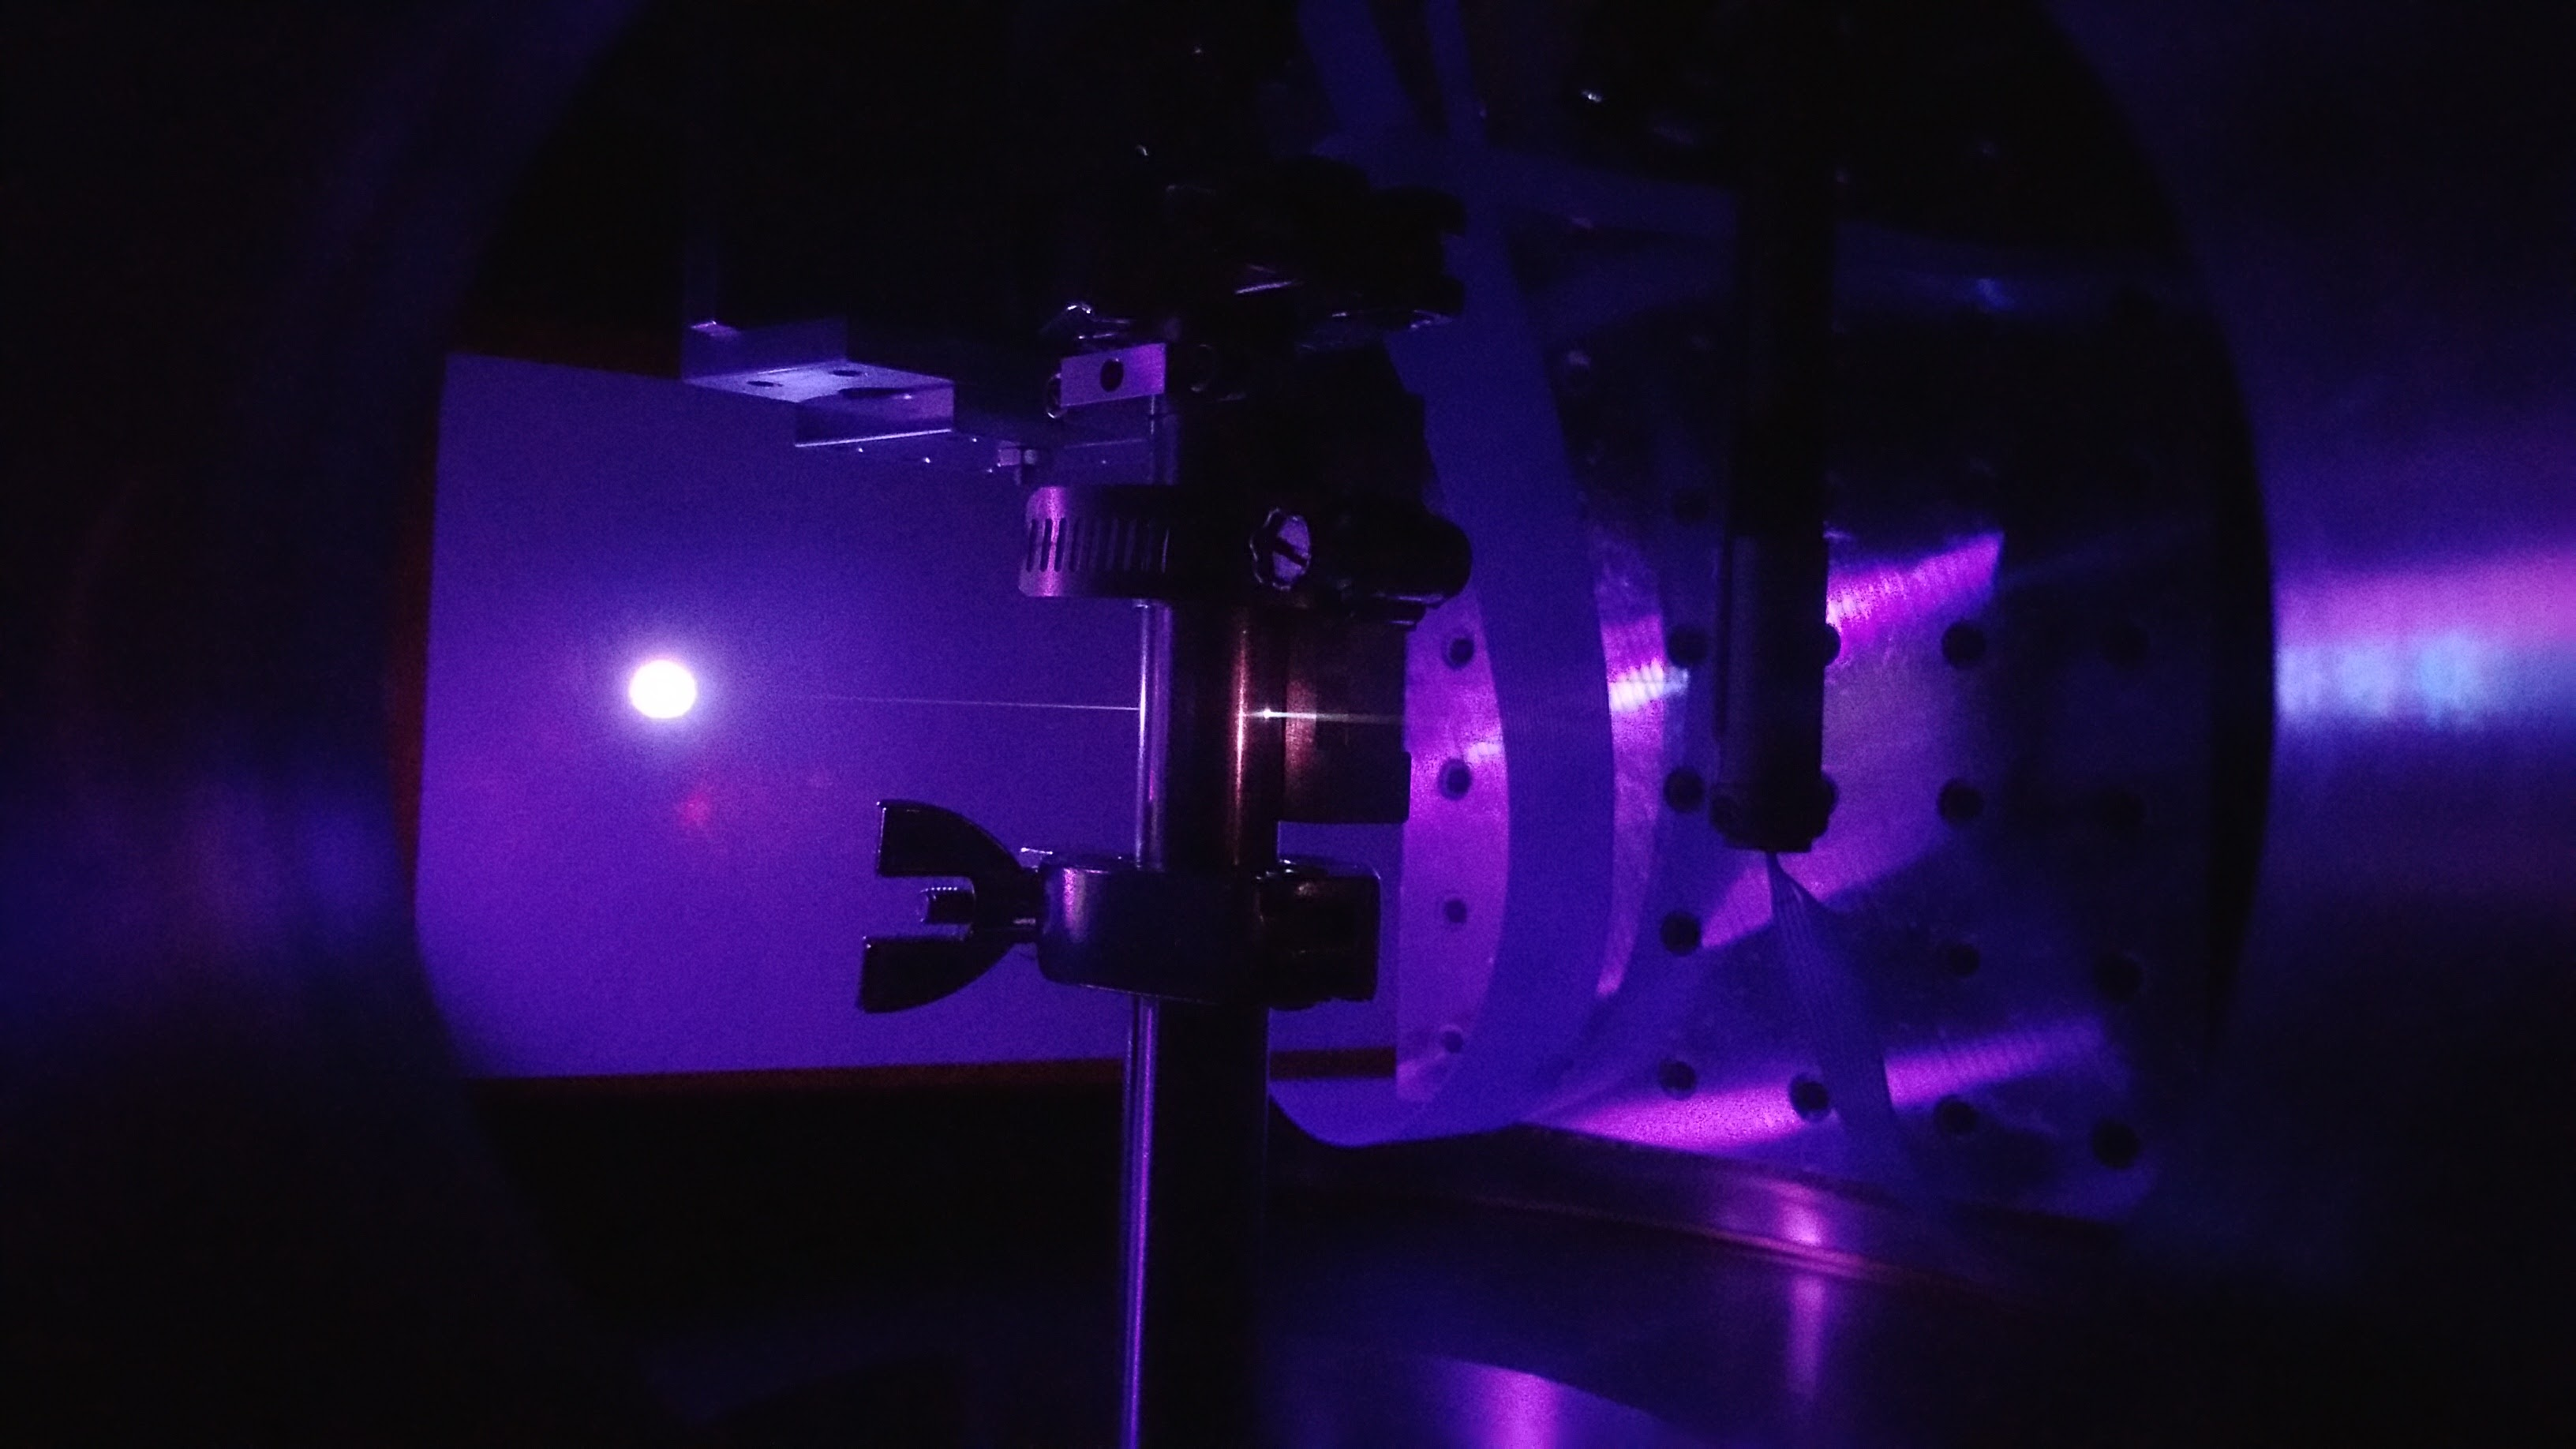
\includegraphics[angle=270, width=0.5\textwidth]{figures/app1/HPC_drilling.jpg}
	\caption{Laser drilling the inner pipe. A card blocks the laser after exiting the HPC. The HPC was pressurized with Ar gas to enhance the filament for illustrative purposes.}
	\label{fig:HPC_drilling}
\end{figure}

\subsection{Introduction}
\textit{main text: description of the HPC's design, pressure \& harmonic performance, pressure modeling, phase matching considerations. this section: how to install and actually use the HPC, how to machine or reorder certain parts.}

- focal length considerations. range of acceptable focal lengths. advantages of reflective vs transmissive focusing. possible schemes for shorter focal lengths. 

- space constraints of TABLe generation chamber limit the size of the XYZ stack. these are Newport 9066 1/2" travel stages, with 1" travel thorlabs motors (that's what we had, ideally you would use 1/2" motors). as a result, you can accidentally drive the motor more than the stage will allow. this will result in the motor falling out of the stage. in this case, you will have to immediately block the laser, vent the chamber, and reattach the motor. note: travel of all motors is from 0 to 14 mm.

- in-vacuum manipulation via the vacuum bellows (limits of motion, max pressure differential)

The ancillary vacuum hardware can be seen in Fig \ref{fig:HPC_outside_view}. A small oil-lubricated RV pump (not shown in this picture) provides differential pumping to the interior of the HPC. An inline Baratron diaphragm pressure sensor (effective range: 1 - 760 Torr) tracks the interior pressure of the edge-welded bellows. A manual gate valve is used to isolate the HPC from the RV pump when the additional pumping is not needed. Right angle KF fittings were used to route the HPC's vacuum line above the pump arm of the interferometer.


\subsection{Initial Installation and Alignment}
\label{app:initial-alignment-HPC}
First, a note about laser safety. The following alignment procedure should be done at the lowest possible laser power to minimize both accidental drilling of the HPC and the danger posed by stray light. Stray reflections or scatter from the many metallic surfaces of the HPC assembly pose a potential safety risk during alignment. The surface most likely to cause laser scatter is the front face of the outer pipe, which is roughened stainless steel located about 3/8" before the focus. The material's roughness and the negative radius of curvature of the incoming light make it unlikely that incident light will coherently focus to a point upon reflection. However, it is possible that the sidewall of the outer pipes's aperture could act as a focusing mirror. Additionally, the hose clamp or mounting bracket could coherently reflect light towards the user. The user is advised to strictly follow all laser safety protocols during this alignment procedure. Whenever possible, direct observation of the laser beam on the surfaces of the HPC should be avoided, instead a webcam should be used to view the interior of the generation chamber.

The initial installation of the HPC can be time consuming and tedious, but once installed it will retain its alignment for a period of weeks or months. The pointing into the cell should be done on a daily basis, but this is only slightly more complicated than what must be done with a free expansion gas jet.

Optically, the HPC cell consists of four pinhole apertures (diametrically opposed pinholes on both the inner and outer pipes) with the laser focus near the center of the inner pipe. The optical transmission of the HPC is therefore very sensitive to the relative alignment of these components, as well as the pointing of the laser into the HPC. To simplify the alignment, the two innermost holes are laser drilled \textit{in-situ} after the outer pipe has been aligned. To maintain the relative alignment of the inner \& outer apertures, the user should refrain from adjusting the inner pipe after the initial alignment is completed. Therefore, daily alignment of the HPC should be performed using only the in-vacuum motorized XYZ stages.

The first step of the HPC installation is installing the rough vacuum feedthrough flange. The TABLe's generation chamber uses a custom flange (a 4.5" CF blank with a KF16 half nipple welded to the air-side and a KF16 bulkhead groove \& tapped holes machined into the vacuum side). To accommodate the length of the in-vacuum bellows, we use a custom 10" CF to 4.5" CF reducing nipple (OAL = 4.25"), which acts as a spacer between the feedthrough flange and the KF16 flange on the HPC. Although it was absent from the original design, a spacer 4.5" CF flange (thickness = 0.68") between the feedthrough and the reducing full nipple is used to relax the compression in the bellows and allow for a larger range of motion. For convenience, the user should install the edge-welded bellows to the bulkhead flange before installing the flange on the chamber.

The supporting bracket for the HPC was designed to be interchangeable with the free gas nozzle's bracket. This design, shown in Fig. \ref{fig:HPC_on_stage}, allows the user to change the gas source type without disturbing the alignment of the XYZ stage to the optical axis. For completeness, we will assume that the XYZ stage has been misaligned or removed from the chamber. First, the user should align the laser to the interferometer so that the laser path in the generation chamber can be used as a reference. Then, the stage should be positioned in the chamber so that the focus is roughly in the center of the stage's motion. Finally, the stage's z-direction should made parallel to the optic axis. This can be done by tracking the position of the laser on a card mounted to the stage while moving the stage upstream and downstream of the focus. After clamping the stage to the breadboard, check that the alignment is still true before continuing to the next step.

The next step is to align the outer pipe of the high pressure cell by maximizing its light transmission. This is best done in two steps: first, coarse alignment is done visually at low power (insufficiently intense to laser drill the pipe), followed by fine adjustments using a power meter at moderate intensities (above the noise floor of the power meter). Note that accidentally drilling out the outer pipe will reduce its differential pumping performance. Given the chamber's small size, it is not practical to place a power meter in the generation chamber after the focus during the alignment procedure. Rather, it is preferable to divert the beam out of the vacuum system using the linear actuator \& silver mirror assembly located approximately 85 cm downstream of the focus.\footnote{Special thanks to Eric Moore for designing and installing this optomechanical component.} When inserted, the linear actuator intersects the beam path and redirects the beam out of the vacuum system through a window onto the upper deck of the optical table. The beam size can be reduced using a focusing lens onto the face of a power meter. Note that for most generation focusing conditions, the large beam size at the diverting mirror makes this beam path lossy. To accurately calculate the transmission through the HPC, it is necessary to measure the power immediately after the HPC in the generation chamber.

For the coarse alignment, the input beam intensity should be reduced using an upstream iris, to the point that it is barely visible near the focus. Since a tightened KF connection prevents rotation of the components, the alignment of the outer piper is done prior to making any KF connections. However, the KF clamps should be fitted on either end of the pipe to ensure that there is enough room to make the connections without disturbing the alignment once finished. The outer pipe should be placed in its cradle, with the aluminum \& hose clamps made snug around the pipe but not taut.\footnote{The HPC's XYZ assembly and bracket were designed for the TABLe generation chamber. If it is being installed elsewhere, the user should verify that the height is correct. When installed correctly, the bottom of the Z-motor range should correspond to the HPC lowered completely out of the way of the laser; the top of the range should correspond to the laser going through the center of the HPC, with about 1 mm to spare.} Transmission should be optimized by iteratively tuning the following parameters: (1) rotation of the pipe in the cradle, (2) height of the cradle using the vertical motor, and (3) horizontal (transverse) position of the assembly using both the horizontal motor and the position of the pipe in the cradle. For fine adjustment, the iris should be adjusted so that the power meter reads about 20-30 mW when measured after the linear actuator.\footnote{This power is appropriate for a 1kHz repetition rate and a generation focal length of 30 or 40 cm.} The clamps should be tightened so that movement of the pipe is possible, but difficult. The area around the power meter should be covered to prevent air currents from affecting the measurement. The transmitted power should be optimized using the same procedure as before.

Once the outer pipe is aligned, tighten all connections and connect the bellows to the outer pipe. Check that the alignment has not been changed by torquing these connections. Verify that the unattenuated laser beam can pass through the outer pipe without interference, as shown in Fig. \ref{fig:HPC_outer_can_laser}. If everything looks good, we can proceed to install the inner pipe.

First, attach the gas delivery feedthrough flange onto the HPC assembly without the inner pipe. Being mindful to not disturb the alignment of the outer pipe, check that the gas delivery tubing does not interfere with the laser path. Remove the gas delivery feedthrough flange, cut the inner pipe to length (OAL = 1.75"), and make the Swagelok connection between the inner pipe and the KF feedthrough. Make sure the inner pipe is normal to the flange's sealing surface, otherwise the laser will skim the sidewall of the inner pipe rather than go through the center. Install the gas delivery assembly onto the HPC assembly by tightening the KF clamp.

Laser drilling the inner pipe will sputter a significant amount of metal onto the inner surfaces of the chamber. Since the active drilling surface is on the upstream face of the pipe, most of the material will go upstream. Therefore, the laser window needs to be swapped out for a "sacrificial" window prior to drilling.\footnote{After drilling, the sacrificial window will be completely coated with a thin metal film. Most of the metal can be removed using methanol, but don't expect to be able to use the window for anything but laser drilling. Using a window with different optical properties (i.e., thickness or material), or no window at all, will change the pointing and effective focal length of the beam. It has been suggested that the laser window could be protected by placing a thin sheet of transparent plastic (Saran Wrap) between the window and the HPC, but we haven't tested this method.} Out of an abundance of caution, close the gate valve to the mirror chamber, retract the linear actuator \& silver mirror from the beam path, and block the generation chamber's vacuum aperture with a card.

Laser drilling should be done with the appropriate safety precautions: wearing laser goggles, notifying fellow labmates of your activity, and posting signs on the entrances to the lab. The user can cover up the chamber's flanges and set up a webcam to remotely monitor the laser drilling status to minimize the risk of inadvertent laser exposure.

At this point, the actual process of laser drilling is quite simple. There is no way to control the exact positioning of the inner pipe relative to the outer pipe, so there are no adjustments to make. Rather, the design relies on the mechanical alignment of the inner pipe relative to the outer pipe, which is ultimately set by the gas feedthrough weld, the Swagelok and the KF fitting. On the other hand, a used inner pipe cannot be reinstalled to the HPC once it is removed, since alignment is effectively impossible. To laser drill the pipe, simply let the unattenuated beam into the chamber and wait a few minutes until the laser emerges from the exit of the HPC. See Fig. \ref{fig:HPC_drilling}.

If you are planning on scanning the k-direction of the HPC during an experiment, you should do so now while you are set up for laser drilling. Similarly, if you are using a non-reflective (achromatic) focusing scheme and are planning on changing wavelengths during your experiment (which will change the effective focal length), you should step through the full range of wavelengths while drilling. Doing so will open up the apertures slightly, resulting in additional metal deposition on the sacrificial laser window.

After laser drilling is complete, reinstall the laser window and verify the HPC has retained its alignment.



\subsection{Alignment with the HPC Installed}

The daily pointing procedure, described in \ref{app:pointing-into-TABLE}, is largely unchanged by the presence of the HPC. However, there are some extra considerations that need to be made if the HPC is installed. The small apertures of the HPC and the non-linear nature of HHG demand high accuracy in the pointing into the cell, so small corrections to the positioning of the HPC have to be made after the daily pointing procedure is completed.

\subsubsection{Pointing into the Interferometer}
If the interferometer is already aligned, the presence of the HPC does not really complicate the daily procedure of the beamline. In this case, the user should block the laser into the generation chamber and align the pointing into the interferometer using the pump arm, as usual.\footnote{Failure to block the laser prior to changing the pointing may result in laser-drilling the HPC.} The procedure described in \ref{app:pointing-into-TABLE} is sufficiently accurate to get the laser through the HPC, but it won't necessarily yield optimized harmonics. Rather, the user may have to make small tweaks to the transverse position of the HPC. This can be done by optimizing the harmonic flux by making small (10 - 25 $\mu$m) steps using both the vertical and horizontal HPC motors while monitoring the harmonic yield using a fast camera exposure ($< 0.5$ s). In our experience, the optimal HPC position is typically within 50 $\mu$m of the previous day's position.

The HPC's apertures may no longer be circular if the HPC has been subjected to accidental laser drilling or significant laser drift. Non-circular apertures may result in a complex spatial profile of the harmonics, which can make the optimization of the harmonic yield difficult.

\subsubsection{Aligning the Interferometer}
If the interferometer needs to be realigned, then the HPC must be lowered out of the way of the laser. This is because the spatial mode of the IR is distorted by the HPC's apertures, which can introduce small shifts in the pointing of the IR after the HPC. Once the HPC is out of the way, the alignment procedure described in \ref{app:aligning-interferometer} can be followed without modification. Unless major changes were made to the interferometer, the angle of the HPC's apertures should remain aligned to the k-vector of the generation arm. In this case, the optimal position of the HPC can be found by maximizing the transmitted power of an the attenuated laser through the HPC, as described in the latter part of \ref{app:initial-alignment-HPC}. If major modifications were made to the interferometer, the user should consider aligning the HPC from scratch.


\subsection{Pump Down Procedure}



- pump down procedure

- generating and optimizing harmonics

- max internal pressure / pressure differential of the bellows tube

- max displacement of the tube

\subsection{Startup and Shutdown}


\section{Laser System Specifics}
importance of pointing \& laser performance for our experiments

\subsection{The Spitfire}
\subsubsection{Regular Maintenance}
- cleaning the stretcher

- increasing the pump laser currents

- changing the chiller fluid, desiccants, etc

\subsubsection{quirks and features}
- regen cavity tweaks

- photodiode problems

- software issues - bugs and troubleshooting

\subsection{Pointing Stabilization into the External Compressor}
- dietrich plots for pointing
\subsection{The Spitfire's External Compressor}
\subsubsection{external compressor alignment}
\subsubsection{cleaning the grating}

\subsection{The TOPAS-HE}
- aligning
- importance of power stability and pointing stability

\subsection{stability}
- boxing things up
- power stability throughout the day, people in the lab
- unstable harmonic yield from the HPC at high pressures
\section{The Shutter System}

\section{The Vacuum System}
- blower upgrade

- remote pressure sensing

- vacuum calculations for steady state pressure of beamline

\section{Best practices: data acquisition}

read-out noise from camera. (how noise scales)

\section{Steve's sections}
steve - grating alignment (which axes do what to harmonics?)

steve - 2-source / phase plate stuff, including calibration

steve - operating the cage and crank